\begin{exercice*}
    Pour une bonne partie de pêche au bord de la Moselle, il faut un siège adapté ! Manuel SKOLÈRE est de taille moyenne et ,
    pour être bien assis, il est nécessaire que la hauteur de l'assise de son siège soit comprise entre \Lg{44} et \Lg{46}.

    \begin{minipage}{0.7\linewidth}
        \begin{myBox}{Dimensions d'un siège pliable}
            \begin{itemize}
                \item Longueur des pieds : \Lg{56}.
                \item Largeur de l'assise : \Lg{34}.
                \item Profondeur de l'assise : \Lg{31}.
                \item L'angle $\widehat{ABF}$ est droit.
                \item $ABCD$ est un rectangle.
            \end{itemize}
        \end{myBox}
    \end{minipage}

    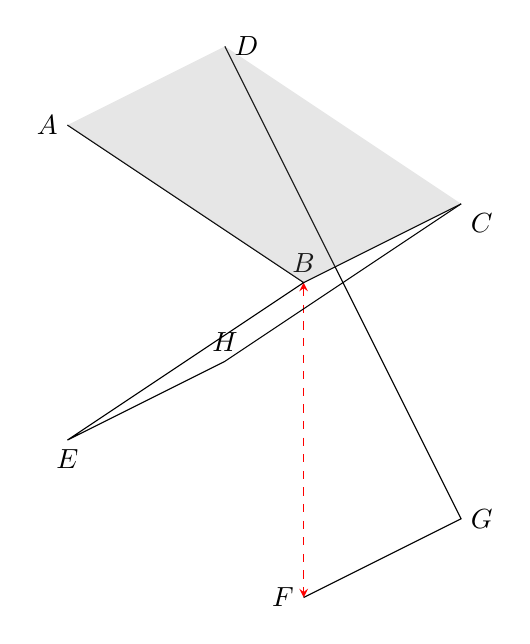
\begin{tikzpicture}[scale=1]
        \coordinate[label=left:$A$] (A) at (1,7);
        \coordinate[label=above:$B$] (B) at (4,5);
        \coordinate[label=below right:$C$] (C) at (6,6);
        \coordinate[label=right:$D$] (D) at (3,8);
        \coordinate[label=below:$E$] (E) at (1,3);
        \coordinate[label=left:$F$] (F) at (4,1);
        \coordinate[label=right:$G$] (G) at (6,2);
        \coordinate[label=above:$H$] (H) at (3,4);
        \begin{scope}[ dim style/.append style={red, dashed},dim fence style/.style={red, dashed}]
            \tkzDrawSegment[dim={\(\Lg{31}\),5mm,sloped,above=1mm}](A,D);
            \tkzDrawSegment[dim={\(\Lg{34}\),5mm,sloped,above=1mm}](D,C);
            \tkzDrawSegment[dim={\(\Lg{56}\),-5mm,sloped,below=1mm,pos=0.4}](A,F);
        \end{scope}
        \draw [stealth-stealth,dashed,red] (B)--(F);
        \tkzLabelSegment[auto,right,red](B,F){??};
        \draw (F)--(G)--(D);
        \draw (A)--(B)--(E)--(H)--(C);
        \draw (B)--(C);
        \fill[gray,opacity=0.2] (A)--(B)--(C)--(D);
        \tkzMarkRightAngle[size=0.4,fill=gray,opacity=0.5](A,B,F);
    \end{tikzpicture}

    Déterminer si la hauteur de ce siège est adaptée à Manuel SKOLÈRE.
\end{exercice*}
\begin{corrige}
    %\setcounter{partie}{0} % Pour s'assurer que le compteur de \partie est à zéro dans les corrigés
    % \phantom{rrr}
    Pour une bonne partie de pêche au bord de la Moselle, il faut un siège adapté ! Manuel SKOLÈRE est de taille moyenne et ,
    pour être bien assis, il est nécessaire que la hauteur de l'assise de son siège soit comprise entre \Lg{44} et \Lg{46}.
    \begin{myBox}{Dimensions d'un siège pliable}
        \begin{itemize}
            \item Longueur des pieds : \Lg{56}.
            \item Largeur de l'assise : \Lg{34}.
            \item Profondeur de l'assise : \Lg{31}.
            \item L'angle $\widehat{ABF}$ est droit.
            \item $ABCD$ est un rectangle.
        \end{itemize}
    \end{myBox}

    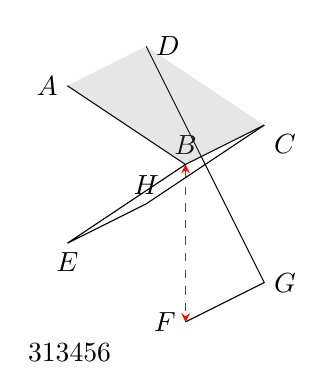
\begin{tikzpicture}[scale=0.5]
        \coordinate[label=left:$A$] (A) at (1,7);
        \coordinate[label=above:$B$] (B) at (4,5);
        \coordinate[label=below right:$C$] (C) at (6,6);
        \coordinate[label=right:$D$] (D) at (3,8);
        \coordinate[label=below:$E$] (E) at (1,3);
        \coordinate[label=left:$F$] (F) at (4,1);
        \coordinate[label=right:$G$] (G) at (6,2);
        \coordinate[label=above:$H$] (H) at (3,4);
        \begin{scope}[ dim style/.append style={red, dashed},dim fence style/.style={red, dashed}]
            \tkzDrawSegment[dim={\(\Lg{31}\),5mm,sloped,above=1mm}](A,D);
            \tkzDrawSegment[dim={\(\Lg{34}\),5mm,sloped,above=1mm}](D,C);
            \tkzDrawSegment[dim={\(\Lg{56}\),-5mm,sloped,below=1mm,pos=0.4}](A,F);
        \end{scope}
        \draw [stealth-stealth,dashed,red] (B)--(F);
        \tkzLabelSegment[auto,right,red](B,F){??};
        \draw (F)--(G)--(D);
        \draw (A)--(B)--(E)--(H)--(C);
        \draw (B)--(C);
        \fill[gray,opacity=0.2] (A)--(B)--(C)--(D);
        \tkzMarkRightAngle[size=0.4,fill=gray,opacity=0.5](A,B,F);
    \end{tikzpicture}

    Déterminer si la hauteur de ce siège est adaptée à Manuel SKOLÈRE.

    {\red Il s'agit de déterminer la longueur $BF$.

    $ABCD$ est un rectangle donc $AB=DC=\Lg{34}$.\\
    \Pythagore[Precision=2]{ABF}{56}{34}{}

    La hauteur de l'assise est comprise entre \Lg{44} et \Lg{46} donc le siège est adapté à Manuel SKOLÈRE.
    }
\end{corrige}

